\documentclass{plt}

\usetheme{metropolis}           % Use metropolis theme

\title{The MicroC Compiler}
\author{Ronghui Gu}
\institute{Columbia University}
\date{Spring 2019}
\titlegraphic{
\vspace{220pt}
{\tiny $^*$ Course website: \url{https://www.cs.columbia.edu/~rgu/courses/4115/spring2019}\vspace{-5pt}}\\
{\tiny $^{**}$ These slides are borrowed from Prof. Edwards.}
}


\lstdefinelanguage{llvm}{
  columns=flexible,
  basicstyle={\fontsize{8.5}{9.5}\selectfont\sffamily\spaceskip=4pt},%
  morekeywords={define,declare,alloca,store,br,label,load,icmp,ne,i1,i8,i32,sgt,add,sub,ret,false,true,global,void,private,unnamed_addr,constant,getelementptr,inbounds,sne,bz,slt,jmp},%
  morecomment=[l]{;},%
}

\lstnewenvironment{llvm}
  {\lstset{language=llvm}\shadowstart}{\shadowend}

\lstnewenvironment{llvm-small}
  {\lstset{language=llvm,basicstyle={\fontsize{6}{5.5}\selectfont\sffamily}}\shadowstart}{\shadowend}

\lstnewenvironment{llvm-stretch}
  {\lstset{language=llvm,basicstyle={\fontsize{9}{16}\selectfont\sffamily}}\shadowstart}{\shadowend}

\tikzset{
    mymodule/.style={draw, fill=white, drop shadow},
    code/.style={draw, fill=gray!15, drop shadow,minimum width=0},
    emph/.style={draw, fill=mBlue!15, drop shadow},
}

\begin{document}

\frame{\titlepage}

%\frame{\tableofcontents}

\begin{frame}[fragile=singleslide]{The MicroC Language}

A very stripped-down dialect of C

Functions, global variables, and some expressions and statements, but
only integer, and boolean values.

\begin{C}
/* The GCD algorithm in MicroC */
int gcd(int a, int b) {
  while (a != b) {
    if (a > b) a = a - b;
    else b = b - a;
  }
  return a;
}

int main() {
  print(gcd(2,14));
  print(gcd(3,15));
  print(gcd(99,121));
  return 0;
}
\end{C}

\end{frame}

\part{Scanning and Parsing}

\begin{frame}[fragile,t]{Scanning and Parsing}

\begin{center}
\hspace{20pt}
\begin{tikzpicture}
  \matrix [matrix of nodes,
           row sep=0.8pc,
           column sep=2pc,
           every node/.style={draw, fill=white, drop shadow,minimum width=5.5cm}] {
     |[code] (b)| MicroC \\
     |[emph] (a)| Lexical Analysis \\
     |[emph] (aa)| Syntax  Analysis \\
     |(aaa)| Semantic Analysis \\
     |(a4)| Intermediate Code Generation \\
     |[code] (a5)| LLVM IR \\
  };
  \begin{scope}[->]
    \draw (b) -- (a);
    \draw (a) -- (aa);
    \draw (aa) -- (aaa);
    \draw (aaa) -- (a4);
    \draw (a4) -- (a5);
  \end{scope};
  \node at (9pc,0) {front-end};
\end{tikzpicture}

Tokenize and parse to produce 
an Abstract Syntax Tree \\
\medskip
The first part of any compiler or interpreter
\end{center}
\end{frame}

\begin{frame}[fragile=singleslide]{The Scanner (scanner.mll)}

  \begin{columns}
    \begin{column}{\dimexpr\textwidth+3pc}
\begin{ocamllex}
{ open Microcparse }  
let digit = ['0' - '9']

rule token = parse
  [' ' '\t' '\r' '\n'] { token   lexbuf }
| "/*"                 { comment lexbuf }          
| "if"     { IF }     | '(' { LPAREN } | '='  { ASSIGN } 
| "else"   { ELSE }   | ')' { RPAREN } | "==" { EQ }    | ">"  { GT }    
| "for"    { FOR }    | '{' { LBRACE } | "!=" { NEQ }   | ">=" { GEQ }   
| "while"  { WHILE }  | '}' { RBRACE } | '<'  { LT }    | "&&" { AND }   
| "return" { RETURN } | ';' { SEMI }   | "<=" { LEQ }   | "||" { OR }    
| "int"    { INT }    | '+' { PLUS }   | ','  { COMMA } | "!"  { NOT } 
| "bool"   { BOOL }   | '-' { MINUS }  | "true"   { BLIT(true)  }
| "float"  { FLOAT }  | '*' { TIMES }  | "false"  { BLIT(false) }
| "void"   { VOID }   | '/' { DIVIDE }                         
| digit+ as lxm { LITERAL(int_of_string lxm) }
| digit+ '.' digit* (['e' 'E'] ['+' '-']? digits)? as lxm { FLIT(lxm) }
| ['a'-'z' 'A'-'Z']['a'-'z' 'A'-'Z' '0'-'9' '_']*  as lxm { ID(lxm)   }
| eof { EOF }
| _ as ch { raise (Failure("illegal character " ^ Char.escaped ch)) }

and comment = parse
  "*/" { token lexbuf }
| _    { comment lexbuf }
\end{ocamllex}
    \end{column}
  \end{columns}
\end{frame}

\begin{frame}[fragile=singleslide]{The AST (ast.ml)}

\begin{ocaml}
type op   = Add | Sub | Mult | Div | Equal | Neq | Less | Leq
          | Greater | Geq | And | Or
type uop  = Neg | Not
type typ  = Int | Bool | Float | Void
type bind = typ * string

type expr = Literal of int | Fliteral of string | BoolLit of bool
          | Id      of string
          | Binop   of expr * op * expr | Unop of uop * expr
          | Assign  of string * expr
          | Call    of string * expr list
          | Noexpr
type stmt = Block  of stmt list
          | Expr   of expr
          | Return of expr
          | If     of expr * stmt * stmt
          | For    of expr * expr * expr * stmt
          | While  of expr * stmt          
type func_decl = { typ     : typ;
                   fname   : string;
                   formals : bind list;
                   locals  : bind list;
                   body    : stmt list;  }

type program = bind list * func_decl list
\end{ocaml}

\end{frame}

\begin{frame}[fragile=singleslide]{The Parser (microcparse.mly)}

\begin{ocamlyacc}
%{ open Ast %}
%token SEMI LPAREN RPAREN LBRACE RBRACE COMMA
%token PLUS MINUS TIMES DIVIDE ASSIGN NOT EQ
%token NEQ LT LEQ GT GEQ AND OR RETURN IF ELSE
%token FOR WHILE INT BOOL FLOAT VOID
%token <int> LITERAL
%token <bool> BLIT
%token <string> ID FLIT
%token EOF

%start program
%type <Ast.program> program

%nonassoc NOELSE
%nonassoc ELSE
%right ASSIGN
%left OR
%left AND
%left EQ NEQ
%left LT GT LEQ GEQ
%left PLUS MINUS
%left TIMES DIVIDE
%right NOT

%%
\end{ocamlyacc}
\end{frame}

\begin{frame}[fragile=singleslide]{Declarations}
\begin{ocamlyacc}
program: decls EOF { $1 }

decls: /* nothing */ { ([], [])               }
     | decls vdecl   { (($2 :: fst $1), snd $1) }
     | decls fdecl   { (fst $1, ($2 :: snd $1)) }

fdecl: typ ID LPAREN formals_opt RPAREN
       LBRACE vdecl_list stmt_list RBRACE {
     { typ = $1; fname = $2; formals = List.rev $4;
       locals = List.rev $7; body = List.rev $8 } }

formals_opt:  /* nothing */ { [] }
           | formal_list    { $1 }

formal_list: typ ID                   { [($1,$2)]     }
           | formal_list COMMA typ ID { ($3,$4) :: $1 }

typ: INT   { Int   }   | BOOL  { Bool  }
   | FLOAT { Float }   | VOID  { Void  }

vdecl_list: /* nothing */    { [] }
          | vdecl_list vdecl { $2 :: $1 }

vdecl: typ ID SEMI { ($1, $2) }
\end{ocamlyacc}
\end{frame}

\begin{frame}[fragile=singleslide]{Statements}

\begin{ocamlyacc}
stmt_list:
    /* nothing */  { [] }
  | stmt_list stmt { $2 :: $1 }

stmt:
    expr SEMI                         { Expr $1               }
    
  | RETURN expr_opt SEMI              { Return $2             }
  
  | LBRACE stmt_list RBRACE           { Block(List.rev $2)    }
  
  | IF LPAREN expr RPAREN stmt %prec NOELSE
                                      { If($3, $5, Block([])) }
					
  | IF LPAREN expr RPAREN stmt ELSE stmt
                                      { If($3, $5, $7)        }
  
  | FOR LPAREN expr_opt SEMI expr SEMI expr_opt RPAREN stmt
                                      { For($3, $5, $7, $9)   }
					
  | WHILE LPAREN expr RPAREN stmt     { While($3, $5)         }
\end{ocamlyacc}
\end{frame}


\begin{frame}[fragile=singleslide]{Expressions}

\begin{ocamlyacc}
expr:
    LITERAL              { Literal($1)            }
  | FLIT                 { Fliteral($1)           }
  | BLIT                 { BoolLit($1)            }
  | ID                   { Id($1)                 }
  | expr PLUS   expr     { Binop($1, Add,   $3)   }
  | expr MINUS  expr     { Binop($1, Sub,   $3)   }
  | expr TIMES  expr     { Binop($1, Mult,  $3)   }
  | expr DIVIDE expr     { Binop($1, Div,   $3)   }
  | expr EQ     expr     { Binop($1, Equal, $3)   }
  | expr NEQ    expr     { Binop($1, Neq,   $3)   }
  | expr LT     expr     { Binop($1, Less,  $3)   }
  | expr LEQ    expr     { Binop($1, Leq,   $3)   }
  | expr GT     expr     { Binop($1, Greater, $3) }
  | expr GEQ    expr     { Binop($1, Geq,   $3)   }
  | expr AND    expr     { Binop($1, And,   $3)   }
  | expr OR     expr     { Binop($1, Or,    $3)   }
  | MINUS expr %prec NOT { Unop(Neg, $2)          }
  | NOT expr             { Unop(Not, $2)          }
  | ID ASSIGN expr       { Assign($1, $3)         }
  | ID LPAREN args_opt RPAREN
                         { Call($1, $3)           }
  | LPAREN expr RPAREN   { $2                     }
\end{ocamlyacc}
\end{frame}


\begin{frame}[fragile=singleslide]{Expressions concluded}

\begin{ocamlyacc}
expr_opt:
    /* nothing */ { Noexpr }
  | expr          { $1 }

args_opt:
    /* nothing */ { [] }
  | args_list  { List.rev $1 }

args_list:
    expr                    { [$1] }
  | args_list COMMA expr { $3 :: $1 }
\end{ocamlyacc}
\end{frame}

\begin{frame}[fragile=singleslide,t]{Testing with menhir}

\begin{interactive}
$ \type{menhir -{}-interpret -{}-interpret-show-cst microcparse.mly}
\type{INT ID LPAREN RPAREN LBRACE ID LPAREN LITERAL RPAREN SEMI RBRACE EOF}
ACCEPT
\end{interactive}

\vspace{-2\baselineskip}

\begin{columns}
\begin{column}{0.2\textwidth}

\begin{C}
int main() {
  print(42);
}
\end{C}

\end{column}
\begin{column}{0.8\textwidth}
\fontsize{8}{7.5}\selectfont
\begin{verbatim}
[program:
  [decls:
    [decls:]
    [fdecl:
      [typ: INT]
      ID
      LPAREN
      [formals_opt:]
      RPAREN
      LBRACE
      [vdecl_list:]
      [stmt_list:
        [stmt_list:]
        [stmt:
          [expr:
            ID
            LPAREN
            [actuals_opt: [actuals_list: [expr: LITERAL]]]
            RPAREN
          ]
          SEMI
        ]
      ]
      RBRACE
    ]
  ]
  EOF
]
\end{verbatim}
\end{column}
\end{columns}
\end{frame}

\begin{frame}[fragile=singleslide,t]{AST for the GCD Example}

\begin{columns}
\begin{column}{0.5\textwidth}
\begin{C}
int gcd(int a, int b) {
  while (a != b)
    if (a > b) a = a - b;
    else b = b - a;
  return a;
}
\end{C}
\end{column}
\begin{column}{0.5\textwidth}
\begin{verbatim}
typ = Int
fname = gcd
formals = [Int a; Int b]
locals = []
body = 
\end{verbatim}
\end{column}
\end{columns}

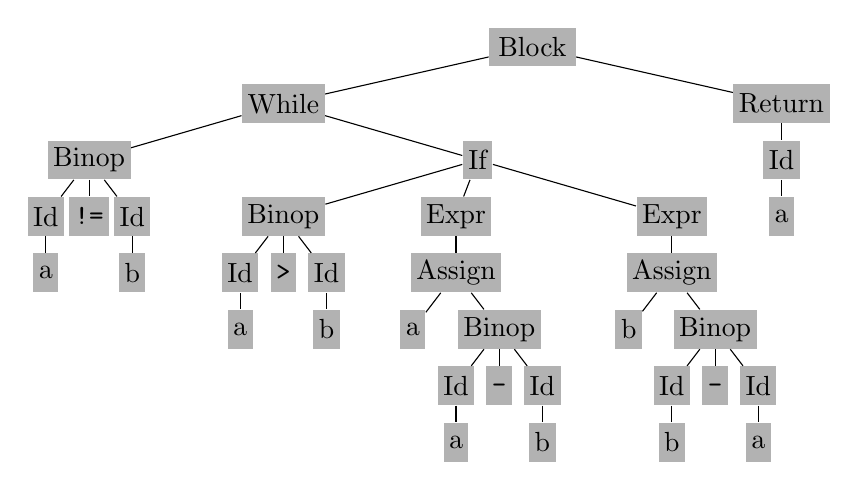
\begin{tikzpicture}
\tikzstyle{every node}=[fill=black!30,minimum height=14pt]
\node {Block} [inner sep=2pt,
               level distance=1.7pc,sibling distance=1.3pc,
               level 1/.style={sibling distance=15pc},
               level 2/.style={sibling distance=1.3pc},
              ]
  child {node {While}
         child {node {Binop}
                child {node {Id} child {node {a}}}
                child {node {\texttt{!=}}}
                child {node {Id} child {node {b}}}}
         child [missing]
         child [missing]
         child [missing]
         child [missing]
         child [missing]
         child [missing]
         child [missing]
         child [missing]
         child {node {If}
                child {node {Binop}
                       child {node {Id} child {node {a}}}
                       child {node {\texttt{>}}}
                       child {node {Id} child {node {b}}}
                      }
                child [missing]
                child [missing]
                child [missing]
                child {node {Expr}
                       child {node {Assign}
                              child {node {a}}
                              child [missing]
                              child {node {Binop}
                                    child {node {Id} child {node {a}}}
                                    child {node {\texttt{-}}}
                                    child {node {Id} child {node {b}}}
                                   }
                             }
                      }
                child [missing]
                child [missing]
                child [missing]
                child [missing]
                child {node {Expr}
                       child {node {Assign}
                              child {node {b}}
                              child [missing]
                              child {node {Binop}
                                    child {node {Id} child {node {b}}}
                                    child {node {\texttt{-}}}
                                    child {node {Id} child {node {a}}}
                                   }
                             }
                      }
               }
         }
   child {node {Return}
          child {node {Id} child {node {a}}}}
;        
\end{tikzpicture}
\end{frame}

\begin{frame}[fragile=singleslide,t]{AST for the GCD Example}

\begin{columns}
\begin{column}{0.5\textwidth}
\begin{C}
int gcd(int a, int b) {
  while (a != b)
    if (a > b) a = a - b;
    else b = b - a;
  return a;
}
\end{C}
\end{column}
\begin{column}{0.5\textwidth}
\begin{verbatim}
typ = Int
fname = gcd
formals = [Int a; Int b]
locals = []
body = 
\end{verbatim}
\end{column}
\end{columns}

\begin{verbatim}
[While (Binop (Id a) Neq (Id b))
       (Block [(If (Binop (Id a) Greater (Id b))
                   (Expr (Assign a
                           (Binop (Id a) Sub (Id b))))
                   (Expr (Assign b
                           (Binop (Id b) Sub (Id a)))))
              ]),
 Return (Id a)]
\end{verbatim}

\end{frame}

\begin{frame}[fragile=singleslide]{Testing the Parser: AST Pretty Printing}

ast.ml has pretty-printing functions; invoke with \texttt{-a}

\begin{interactive}
$ \type{ocamlbuild microc.native}
Finished, 16 targets (0 cached) in 00:00:00.
$ \type{./microc.native -a tests/test-gcd.mc}
int main()
\{
print(gcd(2, 14));
print(gcd(3, 15));
print(gcd(99, 121));
return 0;
\}

int gcd(a,b)
\{
while (a != b) \{
if (a > b)
a = a - b;
else
b = b - a;
\}
return a;
\}
\end{interactive}

\end{frame}

\part{Static Semantic Checking}

\frame{\partpage

\begin{center}
\large
Walk over the AST \\
Verify each node \\
Establish existence of each identifier \\
Establish type of each expression \\
Validate statements in functions
\end{center}

\centerline{\includegraphics[width=0.5\textwidth]{van-de-graff-hair.jpg}}
}

\begin{frame}[fragile]{Static Semantic Analysis}

Lexical analysis: Each token is valid?

\begin{java}
if i 3 "This"                /* valid Java tokens */
#a1123                       /* not a token */
\end{java}

Syntactic analysis: Tokens appear in the correct order?

\begin{java}
for ( i = 1 ; i < 5 ; i++ ) 3 + "foo";  /* valid Java syntax */
for break                               /* invalid syntax */
\end{java}

Semantic analysis: Names used correctly? Types consistent?

\begin{java}
int v = 42 + 13;    /* valid in Java (if v is new) */
return f + f(3);    /* invalid */
\end{java}

\end{frame}


\part{The MicroC Semantic Checker}

\begin{frame}[fragile=singleslide]{The Semantically-Checked AST}
\begin{ocaml}
open Ast
type sexpr = typ * sx    (* The one important change *)
and sx = SLiteral  of int
       | SFliteral of string
       | SBoolLit  of bool
       | SId       of string
       | SBinop    of sexpr * op * sexpr
       | SUnop     of uop * sexpr
       | SAssign   of string * sexpr
       | SCall     of string * sexpr list
       | SNoexpr
type sstmt = SBlock  of sstmt list
           | SExpr   of sexpr
           | SReturn of sexpr
           | SIf     of sexpr * sstmt * sstmt
           | SFor    of sexpr * sexpr * sexpr * sstmt
           | SWhile  of sexpr * sstmt
type sfunc_decl = { styp     : typ;
                    sfname   : string;
                    sformals : bind list;
                    slocals  : bind list;
                    sbody    : sstmt list; }
type sprogram = bind list * sfunc_decl list
\end{ocaml}
\end{frame}

\begin{frame}[fragile=singleslide]{The MicroC Semantic Checker (semant.ml)}

\begin{ocaml}
open Ast
open Sast
module StringMap = Map.Make(String)

(* Some type definitions to clarify signatures *)
type func_symbol = func_decl StringMap.t

(* Semantic checking of the AST. Returns a semantically
   checked program (globals, SAST) if successful;
   throws an exception if something is wrong. *)

let check (globals, functions) =

  (* ... many lines of code .. *) 
  
  in (globals, List.map check_function functions)
\end{ocaml}

\end{frame}

\begin{frame}[fragile=singleslide]{The check\_binds helper function}

Verify a list of bindings has no ``void'' type or duplicate
names.

Used for globals, formal parameters, and local variables.

\begin{ocaml}
let check_binds (kind : string) (binds : bind list) =
  List.iter (function
      (Void, b) -> raise
                    (Failure ("illegal void " ^ kind ^ " " ^ b))
    | _ -> ()) binds;
  let rec dups = function
      [] -> ()
    |	((_,n1) :: (_,n2) :: _) when n1 = n2 ->
        raise (Failure ("duplicate " ^ kind ^ " " ^ n1))
    | _ :: t -> dups t
  in dups (List.sort (fun (_,a) (_,b) -> compare a b) binds)
in  
\end{ocaml}

\end{frame}

\begin{frame}[fragile=singleslide]{Global Variables, Built-in Functions}

\begin{ocaml}
(**** Check global variables ****)

check_binds "global" globals;

(**** Check functions ****)

(* Collect function declarations for built-in functions: no bodies *)
let built_in_decls = 
  let add_bind map (name, ty) = StringMap.add name {
    typ = Void;
    fname = name; 
    formals = [(ty, "x")];
    locals = []; body = [] } map
  in List.fold_left add_bind StringMap.empty [ ("print", Int);
                                               ("printb", Bool);
                                               ("printf", Float);
                                               ("printbig", Int) ]
in
\end{ocaml}

MicroC has 4 built-in functions, \emph{print}, \emph{printb},
\emph{printf}, and \emph{printbig};
this is an easy way to check them.  Your compiler should have very
few exceptions like this.

\end{frame}

\begin{frame}[fragile=singleslide]{Function Symbol Table and ``main''}

\begin{ocaml}
(* Add function name to symbol table *)
let add_func map fd = 
  let built_in_err = "function " ^ fd.fname ^ " may not be defined"
  and dup_err = "duplicate function " ^ fd.fname
  and make_err er = raise (Failure er)
  and n = fd.fname (* Name of the function *)
  (* Prohibit duplicate names or redefinitions of built-ins *)
  in match fd with
       _ when StringMap.mem n built_in_decls -> make_err built_in_err
     | _ when StringMap.mem n map -> make_err dup_err  
     | _ ->  StringMap.add n fd map 
in

(* Collect all function names into one symbol table *)
let function_decls = List.fold_left add_func built_in_decls functions
in

(* Return a function from our symbol table *)
let find_func s = 
  try StringMap.find s function_decls
  with Not_found -> raise (Failure ("unrecognized function " ^ s))
in

(* Ensure "main" is defined *)
let _ = find_func "main" in
\end{ocaml}
\end{frame}

\begin{frame}[fragile=singleslide]{Check a Function}
\begin{ocaml}
let check_function func =
  (* Make sure no formals or locals are void or duplicates *)
  check_binds "formal" func.formals;
  check_binds "local" func.locals;    
\end{ocaml}

A critical helper function for all kinds of assignments:

In the assignment \emph{lvalue} = \emph{rvalue}, \\ can the type of
\emph{rvalue} be assigned to \emph{lvalue}?

In the call \emph{f($\ldots$, arg$_i$, $\ldots$)} where \emph{f} has
formals [$\ldots$, \emph{formal$_i$}, $\ldots$], \\ can
\emph{arg$_i$} be assigned to \emph{formal$_i$}?

\begin{ocaml}
  (* Raise an exception if the given rvalue type cannot
     be assigned to the given lvalue type *)
let check_assign lvaluet rvaluet err =
   if lvaluet = rvaluet then lvaluet else raise (Failure err)
in   
\end{ocaml}

\end{frame}

\begin{frame}[fragile=singleslide]{Variable Symbol Table}

\begin{columns}
\begin{column}{0.4\textwidth}
\parskip=\baselineskip
What can happen when you refer to a variable?

What are MicroC's \emph{scoping rules}?
\end{column}
\begin{column}{0.6\textwidth}
\begin{C}
int a;    /* Global variable */
int c;

void foo(int a) { /* Formal arg. */
  int b;  /* Local variable  */
  ... a = ... a ...
  ... b = ... b ...
  ... c = ... c ...
  ... d = ... d ...
}
\end{C}
\end{column}
\end{columns}

\begin{ocaml}
    (* Variable symbol table: type of each global, formal, local *)
    let symbols = List.fold_left
                   (fun m (t, n) -> StringMap.add n t m)
                   StringMap.empty
                   ( globals @ func.formals @ func.locals )
    in

    (* The key symbol table lookup operation *)
    let type_of_identifier s =
      try StringMap.find s symbols
      with Not_found ->
        raise (Failure ("undeclared identifier " ^ s))
    in
\end{ocaml}
\end{frame}

\begin{frame}[fragile=singleslide]{Expressions}

The expr function: return an SAST sexpr w/type

\begin{ocaml}
(* Return a semantically-checked expression, i.e., with a type *)
let rec expr = function
    Literal  l -> (Int,   SLiteral l)
  | Fliteral l -> (Float, SFliteral l)
  | BoolLit l  -> (Bool,  SBoolLit l)
  | Noexpr     -> (Void,  SNoexpr)
\end{ocaml}

An identifier: does it exist? What is its type?

\begin{ocaml}
  | Id s       -> (type_of_identifier s, SId s)
\end{ocaml}

Assignment: need to know the types of the \emph{lvalue} and
\emph{rvalue}, and whether one can be assigned to the other.

\begin{ocaml}
  | Assign(var, e) as ex -> 
      let lt = type_of_identifier var
      and (rt, e') = expr e in
      let err = "illegal assignment " ^ string_of_typ lt ^ " = " ^ 
        string_of_typ rt ^ " in " ^ string_of_expr ex
      in (check_assign lt rt err, SAssign(var, (rt, e')))
\end{ocaml}
 
\end{frame}

\begin{frame}[fragile=singleslide]{Unary Operators}

  What type is the argument?

\begin{ocaml}
| Unop(op, e) as ex -> 
    let (t, e') = expr e in
    let ty = match op with
      Neg when t = Int || t = Float -> t
    | Not when t = Bool             -> Bool
    | _ -> raise (Failure ("illegal unary operator " ^ 
                           string_of_uop op ^ string_of_typ t ^
                           " in " ^ string_of_expr ex))
    in (ty, SUnop(op, (t, e')))
\end{ocaml}

\end{frame}

\begin{frame}[fragile=singleslide]{Binary Operators}

Check the types of both operands:

\begin{ocaml}
| Binop(e1, op, e2) as e -> 
    let (t1, e1') = expr e1 
    and (t2, e2') = expr e2 in
    (* All binary operators require operands of the same type *)
    let same = t1 = t2 in
    (* Type depends on the operator and types of operands *)
    let ty = match op with
      Add | Sub | Mult | Div when same && t1 = Int   -> Int
    | Add | Sub | Mult | Div when same && t1 = Float -> Float
    | Equal | Neq            when same               -> Bool
    | Less | Leq | Greater | Geq
               when same && (t1 = Int || t1 = Float) -> Bool
    | And | Or when same && t1 = Bool                -> Bool
    | _ -> raise (
        Failure ("illegal binary operator " ^
                 string_of_typ t1 ^ " " ^ string_of_op op ^ " " ^
                 string_of_typ t2 ^ " in " ^ string_of_expr e))
    in (ty, SBinop((t1, e1'), op, (t2, e2')))
\end{ocaml}
\end{frame}

\begin{frame}[fragile=singleslide]{Function Calls}

Number and type of formals and actuals must match

\begin{columns}
\begin{column}{0.5\textwidth}
\begin{C}
void foo(t1 f1, t2 f2) { ... }
\end{C}
\end{column}
\begin{column}{0.5\textwidth}
\begin{C}
... = ... foo(expr1, expr2) ...
\end{C}
\end{column}
\end{columns}

\begin{columns}
\begin{column}{0.4\textwidth}
The callsite behaves like
\end{column}
\begin{column}{0.6\textwidth}
\begin{C}
f1 = expr1;
f2 = expr2;
\end{C}
\end{column}
\end{columns}

\begin{ocaml}
| Call(fname, args) as call -> 
    let fd = find_func fname in
    let param_length = List.length fd.formals in
    if List.length args != param_length then
      raise (Failure ("expecting " ^ string_of_int param_length ^ 
                      " arguments in " ^ string_of_expr call))
    else let check_call (ft, _) e = 
      let (et, e') = expr e in 
      let err = "illegal argument found " ^ string_of_typ et ^
        " expected " ^ string_of_typ ft ^ " in " ^ string_of_expr e
      in (check_assign ft et err, e')
    in 
    let args' = List.map2 check_call fd.formals args
    in (fd.typ, SCall(fname, args'))
\end{ocaml}
\end{frame}

\begin{frame}[fragile=singleslide]{Statements}

Make sure an expression is Boolean: used in \emph{if}, \emph{for}, \emph{while}.

\begin{ocaml}
let check_bool_expr e = 
  let (t', e') = expr e
  and err = "expected Boolean expression in " ^ string_of_expr e
  in if t' != Bool then raise (Failure err) else (t', e') 
in
\end{ocaml}

Checking a statement: make sure it is well-formed and return a
semantically-checked statement (i.e., SAST.sstmt)

\begin{ocaml}
let rec check_stmt = function
    Expr e -> SExpr (expr e)
  | If(p, b1, b2) ->
      SIf(check_bool_expr p, check_stmt b1, check_stmt b2)
  | For(e1, e2, e3, st) ->
      SFor(expr e1, check_bool_expr e2, expr e3, check_stmt st)
  | While(p, s) -> SWhile(check_bool_expr p, check_stmt s)
\end{ocaml}

\end{frame}

\begin{frame}[fragile=singleslide]{Statements: Return}

The type of the argument to \emph{return} must match the type of the function.

\begin{ocaml}
      | Return e -> let (t, e') = expr e in
        if t = func.typ then SReturn (t, e') 
        else raise (
	  Failure ("return gives " ^ string_of_typ t ^ " expected " ^
		   string_of_typ func.typ ^ " in " ^ string_of_expr e))	    
\end{ocaml}

\end{frame}

\begin{frame}[fragile=singleslide]{Statements: Blocks}

Checking a block of statements is almost \verb|List.iter stmt sl|, but
LLVM does not like code after a return:

\begin{C}
int main() {
   return 1;
   print(42); /* Illegal: code after a return */
}
\end{C}

\begin{ocaml}
      | Block sl -> 
          let rec check_stmt_list = function
              [Return _ as s] -> [check_stmt s]
            | Return _ :: _   -> raise (Failure "nothing may follow a return")
            | Block sl :: ss  -> check_stmt_list (sl @ ss) (* Flatten blocks *)
            | s :: ss         -> check_stmt s :: check_stmt_list ss
            | []              -> []
          in SBlock(check_stmt_list sl)
\end{ocaml}

\end{frame}

\begin{frame}[fragile=singleslide]{semant.ml: The Big Picture}

\begin{ocaml}
let check (globals, functions) =
  
  (* check_binds, check globals,
     build and check function symbol table, check for main *)

  let check_function func =

    (* check formal and local bindings *)

    let rec expr = (* ... *) in
  
    let rec check_stmt = (* ... *)

  in { styp     = func.typ;
       sfname   = func.fname;
       sformals = func.formals;
       slocals  = func.locals;
       sbody    = match check_stmt (Block func.body) with 
 	 SBlock(sl) -> sl
       | _ -> raise (Failure
               ("internal error: block didn't become a block?"))
  }
  
in (globals, List.map check_function functions)
\end{ocaml}

\end{frame}


%%%%%%%%%%%%%%%%%%%%%%%%%%%%%%%%%%%%%%%%%%%%%%%%%%%%%%%%%%%%%%%%%%%%%%

\part{The MicroC Code Generator}

\begin{frame}
\partpage

\begin{center}
\large
Assumes AST is semantically correct \\
Translate each AST node into LLVM IR \\
Construct expressions bottom-up \\
Construct basic blocks for control-flow statements \\
\medskip
\url{http://llvm.org} \\
\url{http://llvm.org/docs/tutorial} \\
\medskip
\url{http://llvm.moe} Ocaml bindings documentation
\end{center}

\end{frame}

\begin{frame}[fragile=singleslide]{The Code Generator (codegen.ml)}

The \emph{translate} function takes a semantically checked AST and
returns an LLVM module

\begin{ocaml}
module L = Llvm
module A = Ast
open Sast 

module StringMap = Map.Make(String)

(* translate : Sast.program -> Llvm.module *)
let translate (globals, functions) =
  let context    = L.global_context () in
  
  (* Create the LLVM compilation module into which
     we will generate code *)
  let the_module = L.create_module context "MicroC" in

  (* ... *)  
  let build_function_body fdecl =  
  (* ... *) 
  in
  List.iter build_function_body functions;
  the_module
\end{ocaml}
\end{frame}

\begin{frame}[fragile=singleslide]{The LLVM Type of Types}
  
MicroC only supports primitive types; this could get complicated.
  
\begin{ocaml}
(* Get types from the context *)
let i32_t      = L.i32_type    context
and i8_t       = L.i8_type     context
and i1_t       = L.i1_type     context
and float_t    = L.double_type context
and void_t     = L.void_type   context in

(* Return the LLVM type for a MicroC type *)
let ltype_of_typ = function
    A.Int   -> i32_t
  | A.Bool  -> i1_t
  | A.Float -> float_t
  | A.Void  -> void_t
in    
\end{ocaml}
\end{frame}


\begin{frame}[fragile=singleslide]{Define Global Variables}

\begin{columns}
\begin{column}{0.5\textwidth}
\begin{C}
int i;
bool b;
int k;

int main()
{
  i = 42;
  k = 10;
\end{C}
\end{column}
\begin{column}{0.5\textwidth}
\begin{llvm}
@k   = global i32 0
@b   = global i1 false
@i   = global i32 0

define i32 @main() {
entry:
  store i32 42, i32* @i
  store i32 10, i32* @k
\end{llvm}
\end{column}
\end{columns}

\begin{ocaml}
(* Create a map of global variables after creating each *)
let global_vars : L.llvalue StringMap.t =
  let global_var m (t, n) = 
    let init = match t with
        A.Float -> L.const_float (ltype_of_typ t) 0.0
      | _ -> L.const_int (ltype_of_typ t) 0
    in StringMap.add n (L.define_global n init the_module) m in
  List.fold_left global_var StringMap.empty globals in
\end{ocaml}

\end{frame}

\begin{frame}[fragile=singleslide]{Declare external functions}

Declare \emph{printf}, which we'll use to implement various
\emph{print} functions and \emph{printbig}, which illustrates linking
with external C code

Formal function parameters are passed to LLVM in an OCaml array

\begin{ocaml}
let printf_t : L.lltype = 
    L.var_arg_function_type i32_t [| L.pointer_type i8_t |] in
let printf_func : L.llvalue = 
    L.declare_function "printf" printf_t the_module in

let printbig_t : L.lltype =
    L.function_type i32_t [| i32_t |] in
let printbig_func : L.llvalue =
    L.declare_function "printbig" printbig_t the_module in
\end{ocaml}

\begin{llvm}
declare i32 @printf(i8*, ...)

declare i32 @printbig(i32)
\end{llvm}

\end{frame}

\begin{frame}[fragile=singleslide]{Define function prototypes}

\begin{columns}
\begin{column}{0.5\textwidth}
\begin{C}
void foo() ...

int bar(int a, bool b, int c) ...

int main() ...
\end{C}
\end{column}
\begin{column}{0.5\textwidth}
\begin{llvm}
define void @foo() ...

define i32 @bar(i32 %a, i1 %b, i32 %c) ...

define i32 @main() ...
\end{llvm}
\end{column}
\end{columns}

Build a map from function name to (LLVM function, \emph{fdecl})

Construct the declarations first so we can call them when we build
their bodies.

\begin{ocaml}
(* Define each function (arguments and return type) so we can 
   call it even before we've created its body *)
let function_decls : (L.llvalue * sfunc_decl) StringMap.t =
  let function_decl m fdecl =
    let name = fdecl.sfname
    and formal_types = Array.of_list
         (List.map (fun (t,_) -> ltype_of_typ t) fdecl.sformals)
    in let ftype =
       L.function_type (ltype_of_typ fdecl.styp) formal_types in
    StringMap.add name (L.define_function name ftype the_module,
                        fdecl) m in
  List.fold_left function_decl StringMap.empty functions in
\end{ocaml}
\end{frame}

\begin{frame}[fragile=singleslide]{\emph{build\_function\_body}}

An ``Instruction Builder'' is the LLVM library's object that controls
where the next instruction will be inserted.  It points to some
instruction in some basic block.

This is an unfortunate artifact of LLVM being written in C++.

We also define string constants passed to \emph{printf}.

\begin{ocaml}
(* Fill in the body of the given function *)
let build_function_body fdecl =
  let (the_function, _) =
     StringMap.find fdecl.sfname function_decls in
  let builder =
     L.builder_at_end context (L.entry_block the_function) in

  let int_format_str =
     L.build_global_stringptr "%d\n" "fmt" builder
  and float_format_str =
     L.build_global_stringptr "%g\n" "fmt" builder in
\end{ocaml}

\begin{llvm}
@fmt = private unnamed_addr constant [4 x i8] c"%d\0A\00"
@fmt.1 = private unnamed_addr constant [4 x i8] c"%g\0A\00"
\end{llvm}

\end{frame}

\begin{frame}[fragile=singleslide]{Formals and Locals}

Allocate formal arguments and local variables on the stack; remember
names in \emph{local\_vars} map

\begin{columns}
\begin{column}{0.5\textwidth}
\begin{C}
int foo(int a, bool b)
{
  int c;
  bool d;
\end{C}
\end{column}
\begin{column}{0.5\textwidth}
\begin{llvm}
define i32 @foo(i32 %a, i1 %b) {
entry:
  %a1 = alloca i32
  store i32 %a, i32* %a1
  %b2 = alloca i1
  store i1 %b, i1* %b2
  %c = alloca i32
  %d = alloca i1
\end{llvm}
\end{column}
\end{columns}

\begin{ocaml}    
let local_vars =
  let add_formal m (t, n) p = 
    L.set_value_name n p;
    let local = L.build_alloca (ltype_of_typ t) n builder in
    ignore (L.build_store p local builder);
    StringMap.add n local m
  and add_local m (t, n) =
	let local_var = L.build_alloca (ltype_of_typ t) n builder
	in StringMap.add n local_var m in
	
  let formals = List.fold_left2 add_formal StringMap.empty
    fdecl.sformals (Array.to_list (L.params the_function)) in
  List.fold_left add_local formals fdecl.slocals
\end{ocaml}
\end{frame}

\begin{frame}[fragile=singleslide]{\emph{lookup}}

Look for a variable among the locals/formal arguments, then the
globals.  Semantic checking ensures one of the two is always found.

Used for both identifiers and assignments.

\begin{ocaml}
(* Return the value for a variable or formal argument.
   Check local names first, then global names *)
let lookup n = try StringMap.find n local_vars
               with Not_found -> StringMap.find n global_vars
in
\end{ocaml}

\end{frame}

\begin{frame}[fragile=singleslide]{Expressions}

The main expression function: build instructions in the given builder
that evaluate an expression; return the expression's value

\begin{ocaml}
let rec expr builder ((_, e) : sexpr) = match e with
    SLiteral i     -> L.const_int i32_t i
  | SBoolLit b     -> L.const_int i1_t (if b then 1 else 0)
  | SFliteral l    -> L.const_float_of_string float_t l
  | SNoexpr        -> L.const_int i32_t 0
  | SId s          -> L.build_load (lookup s) s builder
  | SAssign (s, e) -> let e' = expr builder e in
                      ignore(L.build_store e' (lookup s) builder); e'
\end{ocaml}

\begin{columns}
\begin{column}{0.4\textwidth}
\begin{C}
int a;

void foo(int c)
{
  a = c + 42;
}
\end{C}
\end{column}
\begin{column}{0.6\textwidth}
\begin{llvm}
@a = global i32 0

define void @foo(i32 %c) {
entry:
  %c1 = alloca i32
  store i32 %c, i32* %c1
  %c2 = load i32* %c1          ; read c
  %tmp = add i32 %c2, 42       ; tmp = c + 42
  store i32 %tmp, i32* @a      ; a = tmp
  ret void
}
\end{llvm}
\end{column}
\end{columns}

\end{frame}

\begin{frame}[fragile=singleslide]{Binary Operators: Floats}

A trick: if the first operand is a float, treat it as a floating-point
operation

\begin{ocaml}
| SBinop ((A.Float,_ ) as e1, op, e2) ->
    let e1' = expr builder e1
    and e2' = expr builder e2 in
    (match op with 
      A.Add     -> L.build_fadd
    | A.Sub     -> L.build_fsub
    | A.Mult    -> L.build_fmul
    | A.Div     -> L.build_fdiv 
    | A.Equal   -> L.build_fcmp L.Fcmp.Oeq
    | A.Neq     -> L.build_fcmp L.Fcmp.One
    | A.Less    -> L.build_fcmp L.Fcmp.Olt
    | A.Leq     -> L.build_fcmp L.Fcmp.Ole
    | A.Greater -> L.build_fcmp L.Fcmp.Ogt
    | A.Geq     -> L.build_fcmp L.Fcmp.Oge
    | A.And | A.Or ->
    raise (Failure "internal error: semant should have rejected "
           ^ "and/or on float")
    ) e1' e2' "tmp" builder
\end{ocaml}
\end{frame}

\begin{frame}[fragile=singleslide]{Binary Operators: Integers}

Evaluate left and right expressions; combine results

\begin{ocaml}
| SBinop (e1, op, e2) ->
    let e1' = expr builder e1
    and e2' = expr builder e2 in
    (match op with
      A.Add     -> L.build_add
    | A.Sub     -> L.build_sub
    | A.Mult    -> L.build_mul
    | A.Div     -> L.build_sdiv
    | A.And     -> L.build_and
    | A.Or      -> L.build_or
    | A.Equal   -> L.build_icmp L.Icmp.Eq
    | A.Neq     -> L.build_icmp L.Icmp.Ne
    | A.Less    -> L.build_icmp L.Icmp.Slt
    | A.Leq     -> L.build_icmp L.Icmp.Sle
    | A.Greater -> L.build_icmp L.Icmp.Sgt
    | A.Geq     -> L.build_icmp L.Icmp.Sge
    ) e1' e2' "tmp" builder
\end{ocaml}
\end{frame}

\begin{frame}[fragile=singleslide]{neg/not/print/printb}

Unary operators: evaluate subexpression and compute

\begin{ocaml}
| SUnop(op, ((t, _) as e)) ->
    let e' = expr builder e in
    (match op with
      A.Neg when t = A.Float -> L.build_fneg 
    | A.Neg                  -> L.build_neg
    | A.Not                  -> L.build_not) e' "tmp" builder
\end{ocaml}

\end{frame}

\begin{frame}[fragile]{Built-In Functions}

Call external C functions that will be linked in later.

High-Level view of printbig.c:

\begin{C}
#include <stdio.h> //Links in printf
void printbig(int c) {
  /* Code implementing printbig functionality */
}
\end{C}

\emph{print}$\ $/\emph{printb}: Invoke \texttt{printf("\%d$\backslash$n", v)} \\
\emph{printf}: Invoke \texttt{printf("\%g$\backslash$n", v)} \\
\emph{printbig}: Invoke \texttt{printbig(v)}

\begin{ocaml}
| SCall ("print", [e]) | SCall ("printb", [e]) ->
    L.build_call printf_func [| int_format_str ; (expr builder e) |]
                 "printf" builder
| SCall ("printbig", [e]) ->
    L.build_call printbig_func [| (expr builder e) |]
                 "printbig" builder
| SCall ("printf", [e]) -> 
    L.build_call printf_func [| float_format_str ; (expr builder e) |]
                 "printf" builder
\end{ocaml}
\end{frame}

\begin{frame}[fragile=singleslide]{Function calls}

Evaluate the actual arguments right-to-left and pass them to the call.
\emph{Do not name the result of \emph{void} functions.}

\begin{ocaml}
| SCall (f, args) ->
   let (fdef, fdecl) = StringMap.find f function_decls in
   let llargs = List.rev (List.map (expr builder) (List.rev args)) in
   let result = (match fdecl.styp with 
                  A.Void -> ""
                | _ -> f ^ "_result") in
   L.build_call fdef (Array.of_list llargs) result builder
\end{ocaml}

\vspace{-4pt}

\begin{columns}
\begin{column}{0.25\textwidth}
\begin{C}
void foo(int a)
{
  print(a + 3);
}

int main()
{
  foo(40);
  return 0;
}
\end{C}
\end{column}
\begin{column}{0.75\textwidth}
\begin{llvm}
define void @foo(i32 %a) {
entry:
  %a1 = alloca i32
  store i32 %a, i32* %a1
  %a2 = load i32* %a1
  %tmp = add i32 %a2, 3
  %printf = call i32 (i8*, ...)* @printf(i8* getelementptr
    inbounds ([4 x i8]* @fmt1, i32 0, i32 0), i32 %tmp)
  ret void
}
define i32 @main() {
entry:
  call void @foo(i32 40)
  ret i32 0
}
\end{llvm}
\end{column}
\end{columns}

\end{frame}

\begin{frame}[fragile=singleslide]{Statements}

Used to add a branch instruction to a basic block only of one doesn't
already exist.  Used by \emph{if} and \emph{while}

\begin{ocaml}
let add_terminal builder f =
  match L.block_terminator (L.insertion_block builder) with
    Some _ -> ()
  | None -> ignore (f builder) in
\end{ocaml}

The main statement function: build instructions in the given builder
for the statement; return the builder for where the next instruction
should be placed.  Semantic checking ensures \emph{return} has an
expression only in non-void functions

\begin{ocaml}
let rec stmt builder = function
    SBlock sl -> List.fold_left stmt builder sl
  | SExpr e   -> ignore(expr builder e); builder 
  | SReturn e -> ignore(match fdecl.styp with
                          (* Special "return nothing" instr *)
                          A.Void -> L.build_ret_void builder 
                          (* Build return statement *)
                        | _ -> L.build_ret (expr builder e) builder );
                 builder
\end{ocaml}
\end{frame}

\begin{frame}[fragile=singleslide]{\emph{If} Statements}

Build basic blocks for \emph{then}, \emph{else}, and
\emph{merge}---where the next statement will be placed.

\vspace{-2pt}

\begin{columns}
\begin{column}{0.65\textwidth}
\begin{ocaml}
| SIf (predicate, then_stmt, else_stmt) ->
  let bool_val = expr builder predicate in
  let merge_bb = L.append_block context
                   "merge" the_function in
  let b_br_merge = L.build_br merge_bb  in

  let then_bb = L.append_block context
                    "then" the_function in
  add_terminal
   (stmt (L.builder_at_end context then_bb)
         then_stmt)
   b_br_merge;

  let else_bb = L.append_block context
                    "else" the_function in
  add_terminal
   (stmt (L.builder_at_end context else_bb)
         else_stmt)
   b_br_merge;

  ignore(L.build_cond_br bool_val then_bb
                          else_bb builder);
  L.builder_at_end context merge_bb
\end{ocaml}
\end{column}
\begin{column}{0.35\textwidth}

\begin{C}
int cond(bool b) {
  int x;
  if (b) x = 42;
  else   x = 17;
  return x;
}
\end{C}
\includegraphics[width=\textwidth]{llvm-cond-cfg.pdf}
\end{column}
\end{columns}

\end{frame}

\begin{frame}[fragile=singleslide]{\emph{While} Statements}

\begin{columns}
\begin{column}{0.65\textwidth}
\begin{ocaml}
| SWhile (predicate, body) ->
  let pred_bb = L.append_block context
                     "while" the_function in
  ignore(L.build_br pred_bb builder);

  let body_bb = L.append_block context
                "while_body" the_function in
  add_terminal
    (stmt (L.builder_at_end context body_bb)
          body)
    (L.build_br pred_bb);

  let pred_builder =
         L.builder_at_end context pred_bb in
  let bool_val =
              expr pred_builder predicate in

  let merge_bb = L.append_block context
                     "merge" the_function in
  ignore(L.build_cond_br bool_val
             body_bb merge_bb pred_builder);
  L.builder_at_end context merge_bb
\end{ocaml}
\end{column}
\begin{column}{0.35\textwidth}

\begin{C}
int foo(int a)
{
  int j;
  j = 0;
  while (a > 0) {
    j = j + 2;
    a = a - 1;
  }
  return j;
}
\end{C}

\includegraphics[width=\textwidth]{llvm-while-cfg.pdf}

\end{column}
\end{columns}

\end{frame}

\begin{frame}[fragile=singleslide]{\emph{For} Statements: Syntactic Sugar for While}

\begin{columns}
\begin{column}{0.5\textwidth}
\begin{C}
for ( expr1 ; expr2 ; expr3 ) {
  body;
}
\end{C}
\end{column}
\begin{column}{1pc}
$\rightarrow$
\end{column}
\begin{column}{0.4\textwidth}
\begin{C}
expr1;
while ( expr2 ) {
   body;
   expr3;
}
\end{C}
\end{column}
\end{columns}

\begin{ocaml}
      | A.For (e1, e2, e3, body) -> stmt builder
            ( A.Block [A.Expr e1 ;
                       A.While (e2, A.Block [body ;
                                             A.Expr e3]) ] )
    in
\end{ocaml}

\end{frame}


\begin{frame}[fragile=singleslide]{The End}

The remainder of \emph{build\_function\_body}: build the body of the
function by treating it as a block of statements; add a \emph{return}
if control fell off the end

\begin{ocaml}
    (* Build the code for each statement in the function *)
    let builder = stmt builder (SBlock fdecl.sbody) in

    (* Add a return if the last block falls off the end *)
    add_terminal builder (match fdecl.styp with
        A.Void -> L.build_ret_void
      | A.Float -> L.build_ret (L.const_float float_t 0.0)
      | t -> L.build_ret (L.const_int (ltype_of_typ t) 0))
\end{ocaml}

The body of \emph{translate} (shown earlier): build the body of each
function and return the module that was created.

\begin{ocaml}
  in
  List.iter build_function_body functions;
  the_module
\end{ocaml}

\end{frame}

\part{The Top-Level}
\frame{\partpage}

\begin{frame}[fragile=singleslide]{microc.ml (1/2)}

Top-level of the MicroC compiler: handle command-line arguments

\begin{ocaml}
type action = Ast | Sast | LLVM_IR | Compile

let () =
  let action = ref Compile in
  let set_action a () = action := a in
  let speclist = [
    ("-a", Arg.Unit (set_action Ast), "Print the AST");
    ("-s", Arg.Unit (set_action Sast), "Print the SAST");
    ("-l", Arg.Unit (set_action LLVM_IR),
                          "Print the generated LLVM IR");
    ("-c", Arg.Unit (set_action Compile),
      "Check and print the generated LLVM IR (default)");
  ] in  
  let usage_msg = "usage: ./microc.native [-a|-s|-l|-c] [file.mc]" in
  let channel = ref stdin in
  Arg.parse speclist
      (fun filename -> channel := open_in filename) usage_msg;
\end{ocaml}
\end{frame}

\begin{frame}[fragile=singleslide]{microc.ml (2/2)}

  The actual compilation stuff: scan, parse, check the AST, generate
  LLVM IR, dump the module

\begin{ocaml}
  let lexbuf = Lexing.from_channel !channel in
  
  let ast = Microcparse.program Scanner.token lexbuf in
  
  match !action with
    Ast -> print_string (Ast.string_of_program ast)
  | _ -> let sast = Semant.check ast in
    match !action with
      Ast     -> ()

    | Sast    -> print_string (Sast.string_of_sprogram sast)

    | LLVM_IR -> print_string (Llvm.string_of_llmodule
                                  (Codegen.translate sast))

    | Compile -> let m = Codegen.translate sast in
	Llvm_analysis.assert_valid_module m;
	print_string (Llvm.string_of_llmodule m)
\end{ocaml}
\end{frame}

\begin{frame}{Source Code Statistics}
  
\small
  
\begin{tabular}{lrl}
\toprule
\textbf{Source File} & \textbf{Lines} & \textbf{Role} \\
\midrule
scanner.mll   &   50 & Token rules \\
microcparse.mly    &  115 & Context-free grammar \\
ast.ml        &  106 & Abstract syntax tree \& pretty printer \\
sast.ml       &   77 & Post-semantics AST \\
semant.ml     &  188 & Semantic checking \\
codegen.ml    &  245 & LLVM IR generation \\
microc.ml     &   32 & Top-level \\
\midrule
\textbf{Total} & 813 \\
\bottomrule
\end{tabular}

\begin{tabular}{lrr}
\toprule
\textbf{Test Case} & \textbf{Files} & \textbf{Total lines} \\
\midrule
Working .mc & 42 & 539 \\
Working outputs & 42 & 334 \\
Failing .mc & 38 & 332 \\
Error messages & 38 & 38 \\
\midrule
\textbf{Total} & 160 & 1243 \\
\bottomrule
\end{tabular}

\end{frame}



\end{document}

% Local Variables:
% mode: latex
% compile-command: "make microc.pdf"
% End:
